\section{Developing a Quantitative Metric for Evaluating Kernel Security}
\label{sec.metric}

By understanding how lines of code in the kernel are used, we can better predict their
likelihood to contain security flaws. In this section, we formulate and test
a quantitative evaluation metric for securing the OS kernel.
This metric is based on the idea that kernel paths executed by popular applications
during everyday use are less likely to contain security flaws.
%The intuition is that
The rationale is that these code paths are well-tested due to their constant use, and so
fewer bugs can go undetected. Our initial tests yielded promising results, with only one
bug appearing in these popular paths.  We later tested the effectiveness
of our metric against two earlier strategies for predicting bug
locations in the OS kernel, and found our results compared favorably.

\subsection{Experimental Setup}\label{sec-setup}
We used two different versions of
the Linux kernel in our study.
%Since our findings for these versions are quantitatively and qualitatively similar, we report
%the results for 3.13.0 in this section and use 3.14.1 in Section~\ref{sec.evaluation}.
%We used two different versions of Linux kernel, because we want to first establish
%the foundation of our new design with one dataset,
We used version 3.13.0 to test our proposed metric, and evaluated the prototype system based on this
 metric using version 3.14.1 in
Section~\ref{sec.evaluation}. Obtaining results from two different datasets that both validate
our idea ensures that our security metric is unbiased. Furthermore,
it demonstrates the metric is applicable
%not a specifically tailored solution for just one version, but rather
for multiple versions of the Linux kernel.

To trace the kernel, we used \texttt{gcov}~\cite{gcov}, a standard program profiling
tool in the GNU compiler collection (GCC) suite. The tool indicates which lines of kernel
code are executed when an application runs.

\textbf{Popular kernel paths.}
To capture the popular kernel paths, we used two strategies concurrently.
First, we attempted to capture the normal usage behavior of popular applications.
To do this, two students used applications in the 50 most popular Debian
packages~\cite{Top-Packages} (omitting libraries) for Debian 7.0, a widely-used and
popular open source project.
Each student used 25 applications for their designed
tasks (i.e., writing, spell checking, printing in a text editor, or using
an image processing software). In instances where there were two applications that performed a
similar task (i.e., Mozilla Firefox and Google Chrome), both programs were
used. These tests were completed over 20 hours of
total use over 5 calendar days.

The second strategy was to try to capture the total range of applications an
individual computer user might regularly access. The students used the workstation as their
desktop machine for a one-week period. They did their homework, developed
software, communicated with friends and family, and other tasks, using this system.
Software was installed as needed.
%
With the two strategies, we obtained a profile of the lines of
kernel code (publicly available at~\cite{Lind}) that defined our
popular kernel paths.

\textbf{Reachable kernel paths.}
There are certain paths in the kernel, such as unloaded drivers, that are
unreachable and unused.
To make sure that our analysis reflects bug distribution in all reachable paths,
we used two techniques to further examine the reachable lines of
code in the kernel. First,
we performed system call fuzzing with the Trinity
system call fuzz tester~\cite{Trinity}.
%These included 16 child processes
%(Trinity workers) executing each Linux system call with 1 million iterations.
Second, we used the Linux Test Project (LTP)~\cite{LTP}, a test suite written
with detailed kernel knowledge.
%This test suite is meant to exercise the
%existing Linux system call interface to
%test its correctness, robustness, and performance impact.
%
%The (primarily) black box fuzzing from Trinity and test suite of
%LTP combined to reach 44.6\% of the kernel, including all 12.4\% of the popular
%paths.

\textbf{Locating bugs.}
Having identified the kernel paths used in popular applications,
we then investigated how bugs are distributed among these paths. We collected a list of
severe kernel bugs from the National Vulnerability Database~\cite{NVD}.
For each bug, we found the patch that fixed the problem and identified
which lines of kernel code were modified to remove it.
For the purpose of this study, a user program that can execute a line of kernel
code changed by such a patch is considered to have the \textit{potential to
exploit that flaw}.  Note that it is possible that, in some situations, this may
overestimate the ability for an attacker to exploit a flaw, since triggering the
flaw would require executing additional lines of code.

\subsection{Results and Analysis}
\label{Verification-of-Hypothesis}
\begin{figure}
\centering
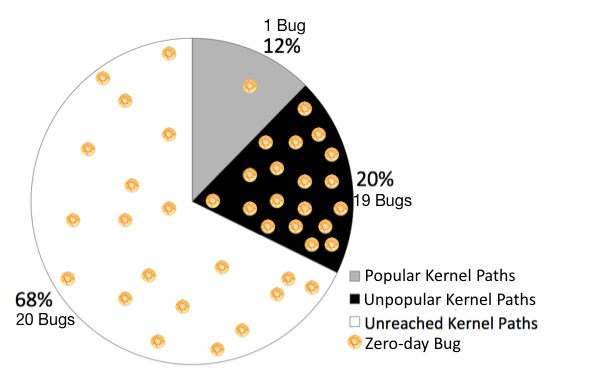
\includegraphics[width=1.0\columnwidth]{diagram/popular_paths.png}
\caption{\small Percentage of different kernel areas that were reached during
 LTP and Trinity system call fuzzing experiments, with the zero-day kernel bugs identified
 in each area.}
\label{fig:coverage}
\end{figure}

%After examining the set of lines that were patched to fix bugs and the traces for
%the commonly-used kernel paths,
The experimental results from Section~\ref{sec-setup} show that only one of the 40 kernel bugs
tested for was found among the popular paths, even though these paths make up 12.4\% of the kernel
(Figure \ref{fig:coverage}).

We then performed a power analysis to test the significance of these results.
%utilizing a Poisson distribution, a form of probability analysis to express the
%likelihood of a given number of events occurring in a fixed interval of time
%and/or space.
%
Our analysis proceeded as follows. We assume that kernel bugs appear at an average rate proportional to the
number of lines of kernel code.
%and different kernel parts may have different rates that bugs appear.
%independently of the time since the last bug occurrence.
Therefore, the rate of defect occurrence per LOC
follows a Poisson distribution~\cite{Poisson-distribution}.
This is consistent with the work of Mayer, et. al.~\cite{mayer1989probability}.
%who proposed a probability model for characterizing the relationship
%between discrete data set.
The premise we tested is that bugs occur at different rates in different
parts of the kernel, i.e., the less popular kernel portion has more bugs.

We first divided the kernel into two sets,
$A$ and $B$, where bugs occur at rates $\lambda_A$ and
$\lambda_B$, and $\lambda_A \neq \lambda_B$. In this test, $A$ is the popular
paths in the kernel, while $B$
represents the less commonly-used paths. Given the null-hypothesis
that the rate of defect occurrences is the \textit{same} in set $A$ and $B$
(or bugs in $A$ and $B$ are drawn from the same Poisson distribution),
we used the Uniformly Most Powerful Unbiased (UMPU) test~\cite{shiue1982experiment}
to compare unequal-sized code blocks.
At a significance level of $\alpha=0.01$, the test was significant at
$\rho=0.0015$, rejecting the null-hypothesis.
The test also reported a 95\% confidence that $\lambda_A / \lambda_B
\in [0.002, 0.525]$. This indicates that the ratio between the bug rates is well
below 1. Since $B$ has a bug rate much larger than that of $A$, it shows 
that $B$ is the risky set containing more bugs. 

The above results show that
popular paths have a much lower bug rate than unpopular ones.
%which means that the popular kernel paths
%contain much fewer bugs. Our metric is thus effective in locating bugs in the Linux kernel.

\subsection{Comparison with Other Security Metrics}

Over the years, a number of metrics for identifying bugs in the OS kernel have
previously been proposed. Most of these security metrics operated at a coarser granularity,
e.g., at the file level. However, when our kernel tests were run at a file
granularity, we found that even popular programs used parts of as many as
32 files that contained flaws. Yet, only one bug was triggered by those programs.
In addition, common programs tested at this level also executed 36 functions
that were later patched to fix security
flaws, indicating the need to localize bugs at a finer granularity.
A few researchers have studied metrics at a finer granularity than file level, which
is at the lines-of-code.
We now discuss two such metrics, and use our Linux kernel version and 40 bugs dataset
to conduct a comparison between them and our popular-paths metric.

\begin{figure}
\centering
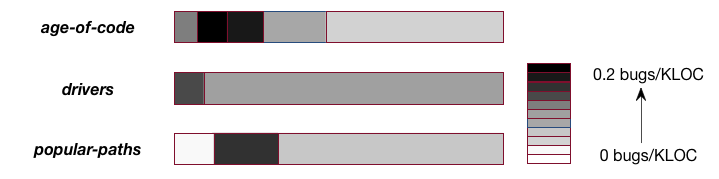
\includegraphics[width=1.2\columnwidth]{diagram/bug_density_v2.png}
\caption{\small Bug density comparison among three metrics.}
\label{fig:bug_density}
\end{figure}

Ozment, et al.~\cite{ozment2006milk} demonstrated that code that
had been around longer in the BSD kernel tended to have fewer bugs.
They determined that a significant extent (61\%) of the reported
vulnerabilities were
%``foundational," meaning they were
introduced prior to the initial version studied.
%They also reported these vulnerabilities have a median lifetime of at least 2.6 years.
To test Ozment's metric using our Linux code and bug dataset,
we separated the code into five different age groups.
Our results (Figure \ref{fig:bug_density}) showed a substantial
number of bugs located in each group, and not just in the newer code.
%No evident cluster patterns among bugs in any particular age group could be identified.
Therefore, buggy code in the Linux kernel cannot be identified simply
by this age-based metric.
In addition, this metric would seem to have limited use for designing a secure
virtualization system. New code is frequently needed to provide
additional functionality,
fix existing problems in the form of patches, and add new technology to improve
user experience. A system could not run very long exclusively on old code.

Another metric, reported by Chou, et al.~\cite{PittSFIeld}, showed that certain parts of the kernel
could be more vulnerable than others. In particular, he identified device drivers as
having much higher error rates.
Applying this metric on our dataset, we found that the driver code in our version
of the Linux kernel accounted for only 8.9\% of the total codebase, and contained
merely 4 out of the 40 bugs (Figure \ref{fig:bug_density}).
One reason for this relatively low number is that, after the Chou study was published,
designers focused efforts on improving driver code. Palix \cite{palix2011faults}
found that, with development of the Linux kernel,
\texttt{drivers} now have lower fault rate than that of other directories,
such as \texttt{arch} and \texttt{fs}.
However, this metric also proves to be difficult to use with the
Linux kernel, since our results show that
only 10.0\% of the kernel bugs could be detected.

To summarize, we demonstrated that both the age-of-code metric and
the drivers metric have weak correlation between the occurrence of bugs
and areas of code they identify. By contrast, our metric of popular
kernel paths provides an effective and statistically significant
%($\alpha=0.01$, $\rho=0.0015$)
means for predicting where in the kernel exploitable flaws
will likely be found. For the remainder of the paper, we will
focus on using this result to design and build secure virtualization systems.
